% file          : doc_tex/basic/Periodic_3_triangulation_3/P3Triang3.tex
% revision      : $Id$
%
% author(s)     : Monique Teillaud <Monique.Teillaud@sophia.inria.fr>
%                 Manuel Caroli <Manuel.Caroli@sophia.inria.fr>

\begin{ccTexOnly}
%\vspace*{-1cm}
\begin{center}
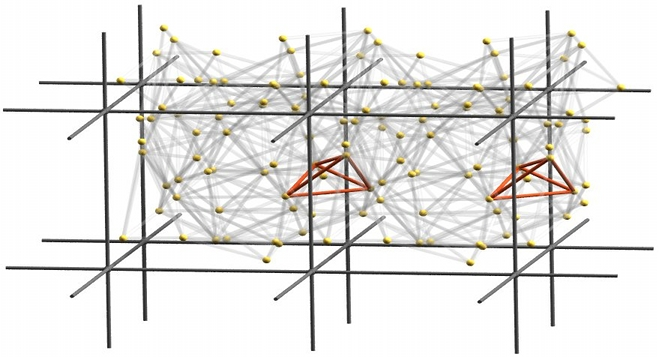
\includegraphics[width=10cm]{Periodic_3_triangulation_3/p3Delaunay3.jpg}
\end{center}
\end{ccTexOnly}
\begin{ccHtmlOnly}
<img border=0 src="./p3Delaunay3.jpg" alt="3D triangulation picture">
\end{ccHtmlOnly}

The periodic 3D-triangulation class of \cgal\ is designed to
represent the triangulations of a set of points in the
three-dimensional flat torus. The triangulation forms a partition of
the space it is computed in. It is a simplicial complex, i.e.\ it
contains all incident $j$-simplices ($j<k$) of any $k$-simplex and two
$k$-simplices either do not intersect or share a common $j$-face,
$j<k$. The occurring simplices of dimension up to three are called
\emph{vertex}, \emph{edge}, \emph{facet}, and \emph{cell}, respectively.

\section{The Flat Torus\label{P3Triangulation3-sec-space}}
The 3D Periodic Triangulation package computes triangulations in the
space $\mathbb T_c^3$, which is defined as follows: Let $c\in\mathbb
R\setminus\{0\}$ and $G$ be the group $(c\cdot\mathbb Z^3, +)$, where
$c\cdot\mathbb Z$ denotes the set containing all integer multiples of
$c$. The flat torus is the quotient space: $\mathbb T_c^3:=\mathbb
R^3/G$. The parameter $c$ defines the period.

The elements of $\mathbb T_c^3$ are the equivalence classes of sets of
points in $\mathbb R^3$. We call these points \textit{representatives}
of an element of $\mathbb 
T_c^3$. The implementation works not directly on elements of $\mathbb
T_c^3$ but on some representatives in $\mathbb R^3$. So there need to
be distinguished representatives to work on. Given $\alpha$, $\beta$,
and $\gamma$, the cube
$[\alpha,\alpha+c)\times[\beta,\beta+c)\times[\gamma,\gamma+c)$ 
contains exactly one representative of each element in $\mathbb
T_c^3$. We call it \emph{original domain}. From now on, when we talk
about \textit{points}, we generally mean representatives of elements
of $\mathbb T_c^3$ that lie inside the original domain. Note that any
input point is required to be an element of the half-open cube
representing the original domain as defined above.

There are simplices containing points inside the original domain but
also points outside it. The points outside the original domain are
periodic copies of points inside the original domain. So, to
specify a simplex we need points together with some additional
information that determines the respective periodic copy of each point. 
The set of representatives of an element of $\mathbb T_c^3$ is a cubic
point grid. We address each representative by a three-dimensional
integer vector $(o_x,o_y,o_z)$, called \emph{offset}. It
represents the number of periods a representative in the original
domain must be translated in $x$-, $y$-, and $z$-direction.
The vector $(0,0,0)$ corresponds to the representative in the original
domain. To specify a $k$-simplex we need $k+1$ point-offset pairs
(cf.\ Fig.~\ref{P3Triangulation3-fig-offsets}). 

\begin{figure}[htbp]
\begin{ccTexOnly}
\begin{center} 
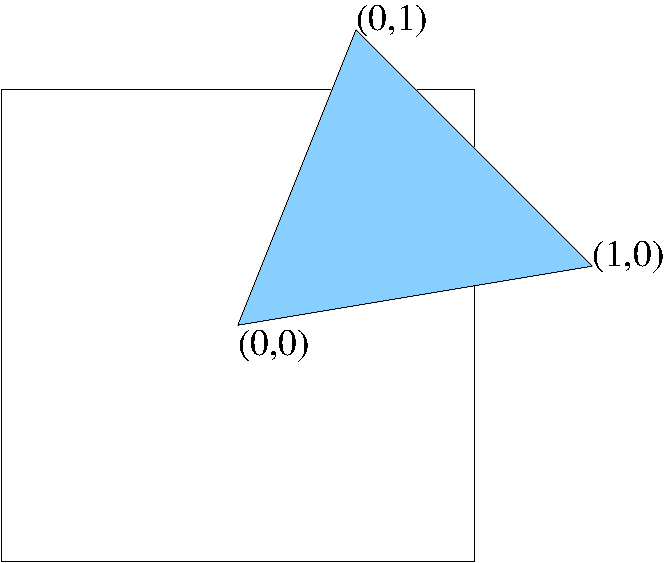
\includegraphics[width=7cm]{Periodic_3_triangulation_3/offsets} 
\end{center}
\end{ccTexOnly}
\begin{ccHtmlOnly}
<CENTER>
<img border=0 src="./offsets.gif" align=middle alt="Offsets in a cell">
</CENTER>
\end{ccHtmlOnly}
\caption{Offsets in a cell.
\label{P3Triangulation3-fig-offsets}}
\end{figure} 

\section{Representation\label{P3Triangulation3-sec-intro}}

A triangulation is a collection of vertices and cells that are linked
together through incidence and adjacency relations. Each cell gives
access to its four incident vertices, their corresponding offsets, and
to its four adjacent cells. Each vertex gives access to one of its
incident cells.

The four vertices of a cell are indexed with 0, 1, 2 and 3 in positive
orientation. The orientation of a simplex in $\mathbb T_c^3$ is
defined as the orientation of the corresponding simplex in $\mathbb
R^3$ given by representatives determined by the respective offsets
(see Figure~\ref{P3Triangulation3-fig-orient}).

\begin{figure}[htbp]
\begin{ccTexOnly}
\begin{center} 
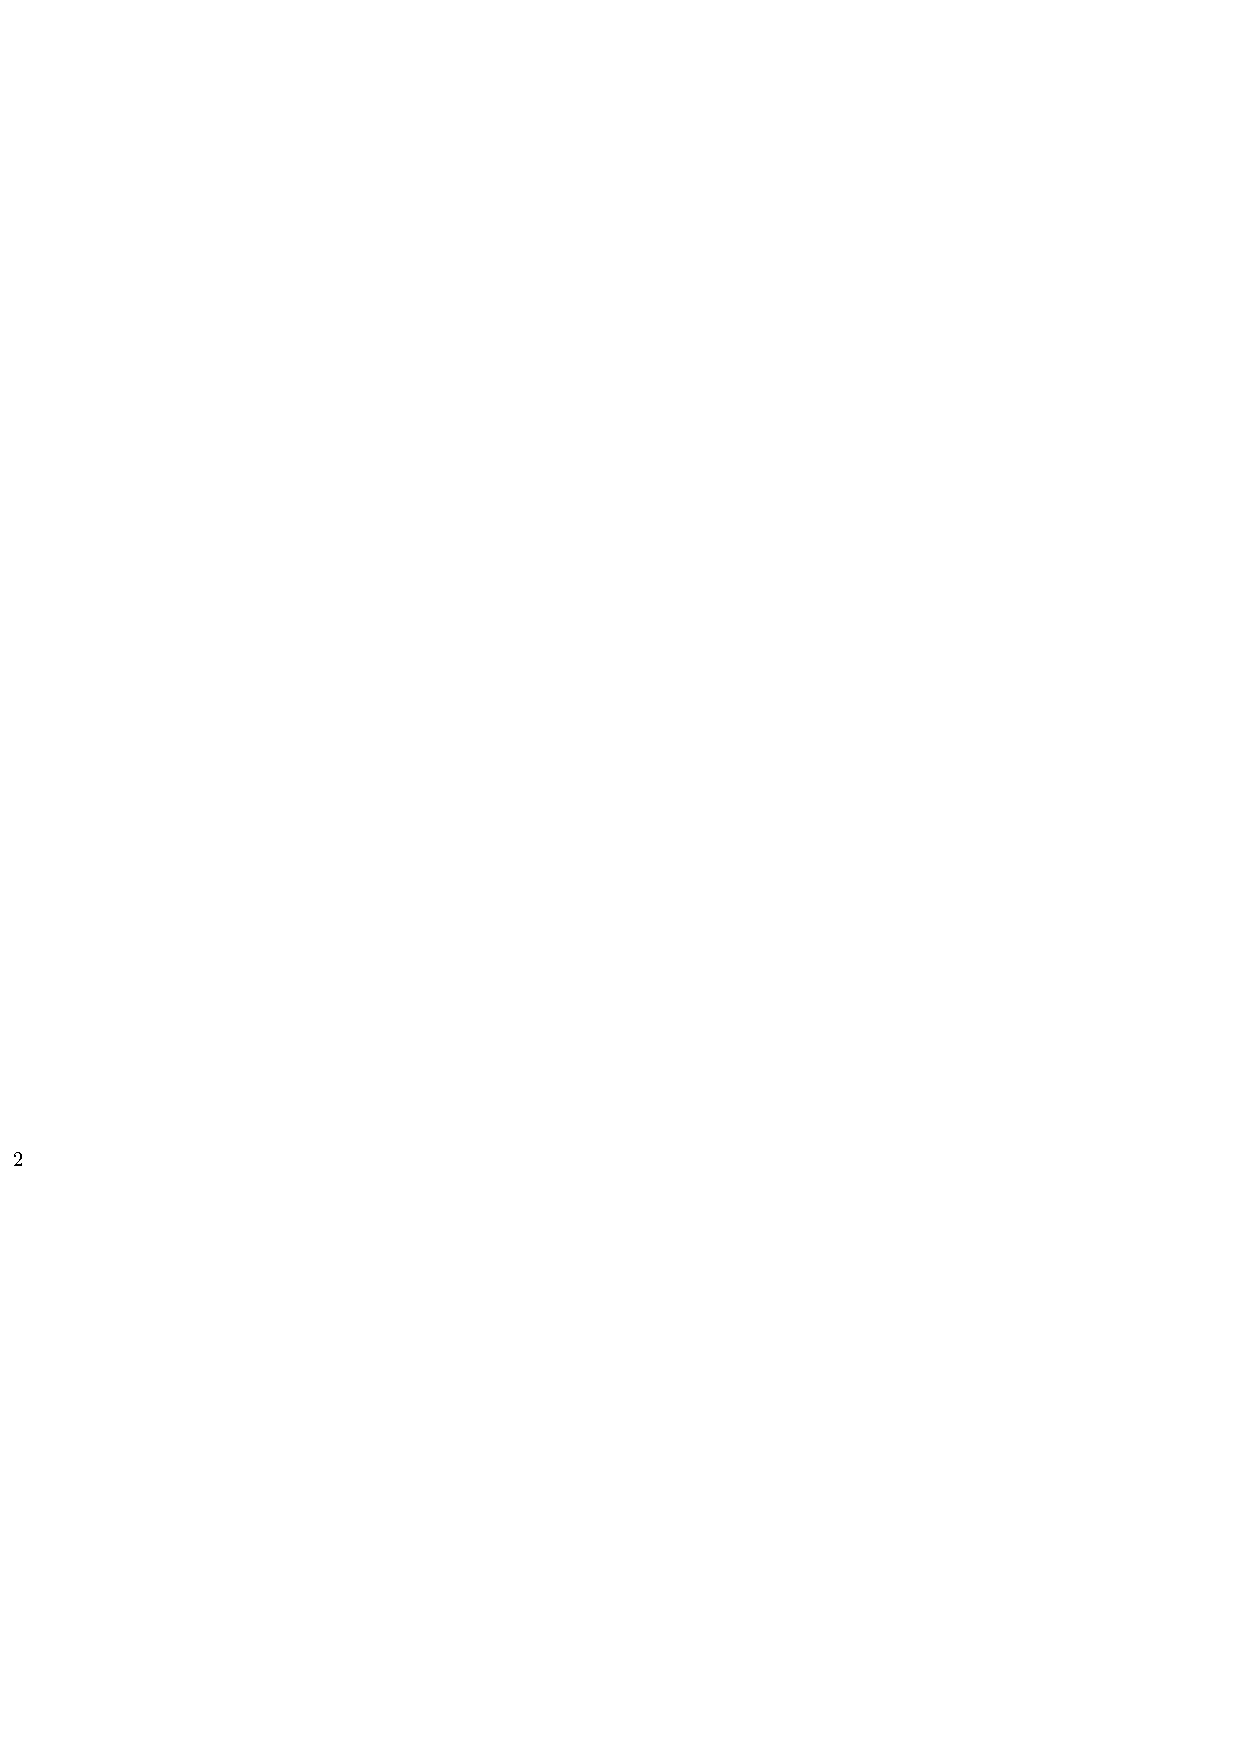
\includegraphics[width=7cm]{Periodic_3_triangulation_3/orient} 
\end{center}
\end{ccTexOnly}
\begin{ccHtmlOnly}
<CENTER>
<img border=0 src="./orient.gif" align=middle alt="Orientation of a cell">
</CENTER>
\end{ccHtmlOnly}
\caption{Orientation of a cell.
\label{P3Triangulation3-fig-orient}}
\end{figure} 

As in the underlying combinatorial triangulation (see
Chapter~\ref{chapter-TDS3}), the neighbors of a cell are indexed with
0, 1, 2, 3 in such a way that the neighbor indexed by $i$ is opposite
to the vertex with the same index. Also edges ($1$-faces) and facets
($2$-faces) are not explicitly represented: a facet is given by a cell
and an index (the facet \ccc{i} of a cell \ccc{c} is the facet of
\ccc{c} that is opposite to the vertex with index \ccc{i}) and an edge
is given by a cell and two indices (the edge \ccc{(i,j)} of a cell
\ccc{c} is the edge whose endpoints are the vertices of \ccc{c} with
indices \ccc{i} and \ccc{j}). See Figure~\ref{TDS3-fig-repres}.  

Some point sets do not admit a triangulation in $\mathbb T_c^3$. In
this case we use 27 periodic copies of the point set arranged in a
cube of edge length $3c$. Any point set constructed in this way has a
triangulation in $\mathbb R^3/G'$ with $G'=((3c\cdot\mathbb Z)^3,+)$
\cite{cgal:ct-c3pt-09}. So we compute the triangulation in this
space, which is a \emph{27-sheeted covering space} of $\mathbb T_c^3$
(see Figure~\ref{P3Triangulation3-fig-covering}).

\begin{figure}[htbp]
\begin{ccTexOnly}
\begin{center} 
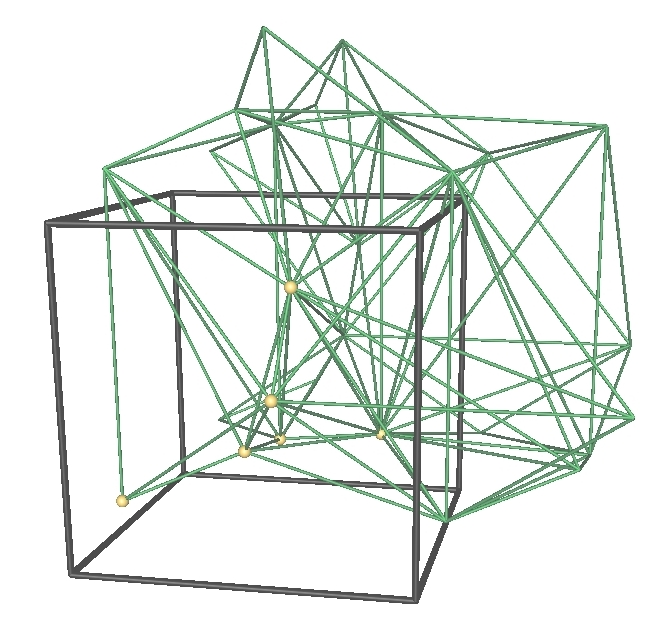
\includegraphics[width=5cm]{Periodic_3_triangulation_3_ref/it_UNIQUE} 
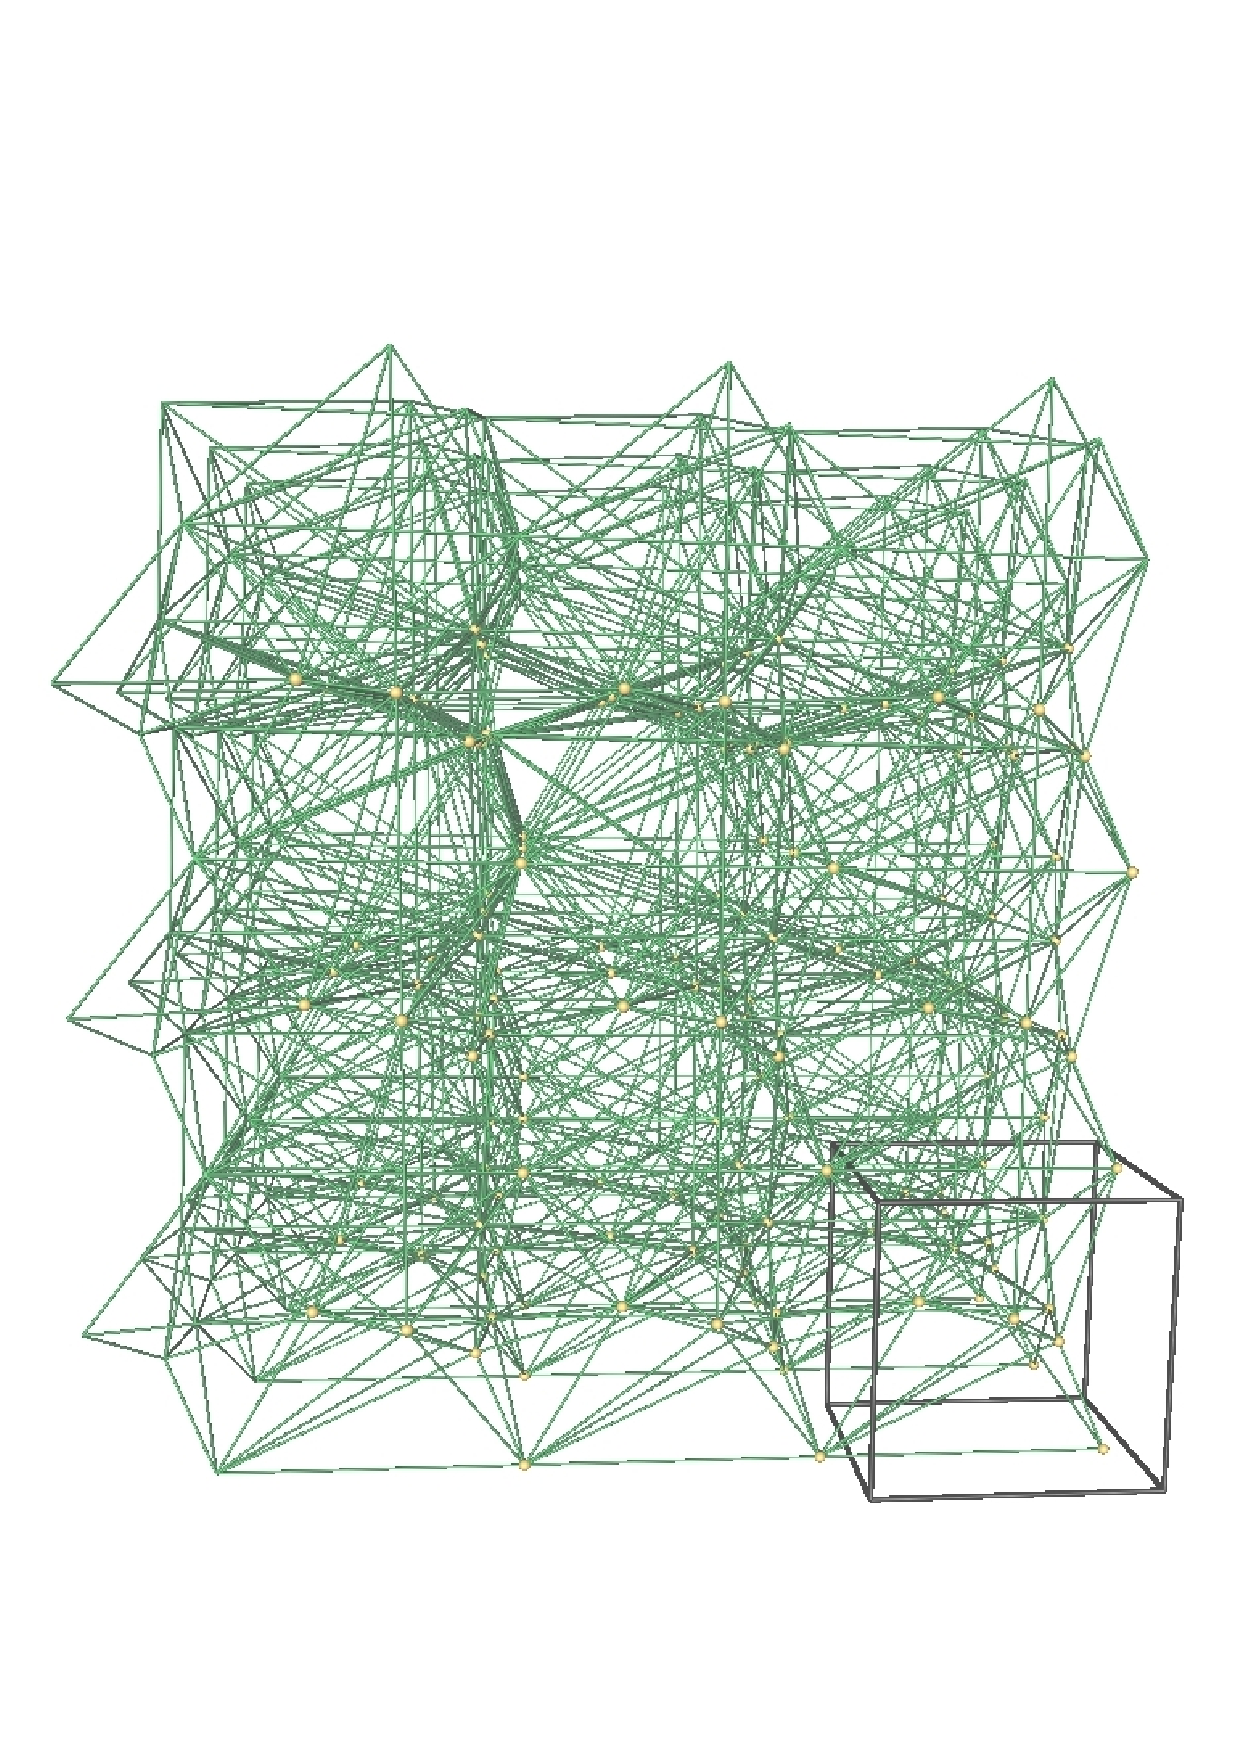
\includegraphics[width=5cm]{Periodic_3_triangulation_3_ref/it_STORED}
\end{center}
\end{ccTexOnly}
\begin{ccHtmlOnly}
<CENTER>
<img border=0 src="../Periodic_3_triangulation_3_ref/it_UNIQUE_small.jpg"
 align=middle alt="UNIQUE">
<img border=0 src="../Periodic_3_triangulation_3_ref/it_STORED_small.jpg"
  align=middle alt="STORED">
</CENTER>
\end{ccHtmlOnly}
\caption{The same periodic triangulation in the 1-sheeted covering space
  and the 27-sheeted covering space.
\label{P3Triangulation3-fig-covering}}
\end{figure} 

The machinery that manages the copies is largely hidden from the
user. However there are some effects that cannot be ignored. For
example if the point set does not permit a triangulation in $\mathbb
T_c^3$ then the combinatorial iterators (\ccc{Cell_iterator},
\ccc{Facet_iterator}, \ccc{Edge_iterator}, and \ccc{Vertex_iterator})
return all simplices that are internally stored, which correspond to
27 periodic copies of each geometric primitive (Tetrahedron, Triangle,
Segment, and Point). This is necessary to ensure consistency in the
adjacency relations. In case it is desired to have only one periodic
copy of each primitive, we provide \emph{geometric} iterators. They
return geometric primitives of the triangulation without relations
between them. Another effect is that when the algorithm switches from
the 27-sheeted covering space to the 1-sheeted covering space, the \ccc{Vertex_handle}s and
\ccc{Cell_handle}s referencing deleted items become invalid.

In the data structure each vertex stores the input point it
corresponds to. If we are computing in the 27-sheeted covering 
space, each vertex stores the representative \emph{inside} the
original domain it corresponds to. So, the 27 vertices corresponding
to the same element of $\mathbb T_c^3$ all store the same
representative in $\mathbb R^3$, and not different periodic copies.

\paragraph{Validity}
A periodic triangulation is said to be \ccc{locally valid} iff

{\bf (a)-(b)} Its underlying combinatorial graph, the triangulation
data structure, is \ccc{locally valid} 
(see Section~\ref{TDS3-sec-intro} of Chapter~\ref{chapter-TDS3})\\
{\bf (c)} Any cell has its vertices ordered according to positive
orientation. See Figure~\ref{P3Triangulation3-fig-orient}.

\section{Delaunay Triangulation} 
The class \ccc{Periodic_3_Delaunay_triangulation_3} implements Delaunay
triangulations of point sets in $\mathbb T_c^3$.

Delaunay triangulations have the \textit{empty sphere property},
that is, the circumscribing sphere of each cell does not contain any
other vertex of the triangulation in its interior. These
triangulations are uniquely defined except in degenerate cases where
five points are co-spherical.  Note however that the \cgal\
implementation computes a unique triangulation even in these cases
\cite{cgal:dt-pvr3d-03}.

This implementation is fully dynamic: it supports both insertions of
points and vertex removal.

\section{Triangulation Hierarchy}
The class \ccc{Periodic_3_triangulation_hierarchy_3} is the adaptation
of the hierarchical structure described in
chapter~\ref{chapter-Triangulation3} to the periodic case.

\section{Software Design\label{P3Triangulation3-sec-design}}
We have chosen the prefix ``Periodic\_3'' to emphasize that the
triangulation is periodic in all three directions of space. There are
also ``cylindrical'' periodicities where the triangulation is periodic
only in one or two directions of space.

The two main classes \ccc{Periodic_3_Delaunay_triangulation_3} and
\ccc{Periodic_3_triangulation_3} provide high-level geometric
functionality and are responsible for the geometric validity.
\ccc{Periodic_3_Delaunay_triangulation_3} contains all the
functionality that is special to Delaunay triangulations, such as
point insertion and vertex removal, the side-of-sphere test, finding
the conflicting region of a given point, dual functions etc.
\ccc{Periodic_3_triangulation_3} contains all the functionality
that is common to triangulations in general, such as location of a
point in the triangulation \cite{cgal:dpt-wt-02}, access functions,
geometric queries like the orientation test etc.

They are built as layers on top of a triangulation data structure,
which stores their combinatorial structure. This separation between
the geometry and the combinatorics is reflected in the software design
by the fact that the triangulation classes take two template
parameters: 
\begin{itemize}
\item {} the \textbf{geometric traits} class, which provides the type of points
to use as well as the elementary operations on them (predicates and
constructions). Furthermore it contains the offset type.
The concept for this parameter is described in more
detail in Section~\ref{P3Triangulation3-sec-Traits}
and as the concept \ccc{Periodic_3DelaunayTriangulationTraits_3} in
the reference
manual\lcTex{ on~\ccRefPage{Periodic_3DelaunayTriangulationTraits_3}}.
\item {} the \textbf{triangulation data structure} class, which stores the
combinatorial structure, described in
Section~\ref{P3Triangulation3-sec-tds} and in more detail in
Chapter~\ref{chapter-TDS3}. The triangulation data structure needs
models of the concepts \ccc{Periodic_3TriangulationDSCellBase_3} and
\ccc{Periodic_3TriangulationDSVertexBase_3} as template parameters. 
\end{itemize}

\subsection{The Geometric Traits Parameter\label{P3Triangulation3-sec-Traits}}
The first template parameter of the Delaunay triangulation class
\ccc{Periodic_3_Delaunay_triangulation_3<Periodic_3DelaunayTriangulationTraits_3, TriangulationDataStructure_3>}
is the geometric traits class, described by the concept
\ccc{Periodic_3DelaunayTriangulationTraits_3}.  It is different to the
DelaunayTriangulationTraits\_3 (see
chapter~\ref{Triangulation3-sec-Traits}) in that it 
implements all objects, predicates and constructions with
using offsets.

The class \ccc{Periodic_3_triangulation_traits_3<Traits,Periodic_3Offset_3>}
provides the required functionality. It expects two template
parameters: A model of the concept \ccc{DelaunayTriangulationTraits_3}
and a model of the concept \ccc{Periodic_3Offset_3}.

The kernels \ccc{Cartesian}, \ccc{Homogeneous},
\ccc{Simple_cartesian}, \ccc{Simple_homogeneous} and
\ccc{Filtered_kernel} can all be used as models for
\ccc{Traits}. \ccc{Periodic_3_triangulation_traits_3} provides exact
predicates and exact constructions if \ccc{Traits} does. It provides
exact predicates but not exact constructions if
\ccc{Filtered_kernel<CK>} with \ccc{CK} an inexact kernel is used as
its first template parameter. Using
\ccc{Exact_predicates_inexact_constructions_kernel}\lcTex{
  (\ccRefPage{Exact_predicates_inexact_constructions_kernel})} as
\ccc{Traits} provides fast and exact predicates and not exact constructions,
using \ccc{Exact_predicates_exact_constructions_kernel}\lcTex{
  (\ccRefPage{Exact_predicates_exact_constructions_kernel})} provides
fast and exact predicates and exact constructions. The latter is recommended if
the dual constructions and constructions of points, segments,
triangles, and tetrahedra are used.

The second parameter \ccc{Periodic_3Offset_3} defaults to
\ccc{Periodic_3_offset_3}.

\subsection{The Triangulation Data Structure Parameter\label{P3Triangulation3-sec-tds}}

The second template parameter of the main classes
\ccc{Periodic_3_triangulation_3} and
\ccc{Periodic_3_Delaunay_triangulation_3} is a
triangulation data structure class.  This class can be seen as a container for
the cells and vertices maintaining incidence and adjacency relations (see
Chapter~\ref{chapter-TDS3}).  A model of this triangulation data structure is
\ccc{Triangulation_data_structure_3}, and it is described by the
\ccc{TriangulationDataStructure_3} concept.  This model is itself
parameterized by a vertex base class and a cell base class, which gives the
possibility to customize the vertices and cells used by the triangulation data
structure, and hence by the geometric triangulation using it.
To represent periodic triangulations the cell base and vertex base
classes need to meet the concepts
\ccc{Periodic_3TriangulationDSCellBase_3} and
\ccc{Periodic_3TriangulationDSVertexBase_3}.

A default value for the triangulation data structure parameter is provided in
all the triangulation classes, so it does not need to be specified by
the user unless he wants to use a different triangulation data
structure or a different vertex or cell base class.

\subsection{Flexibility of the Design}
\ccc{Periodic_3_triangulation_3} uses the
\ccc{TriangulationDataStructure_3} in essentially the same way as
\ccc{Triangulation_3}. That is why the flexibility described in
\ref{Triangulation3-sec-design} is applicable in exactly the same
way. Also the classes \ccc{Triangulation_vertex_base_with_info_3} and
\ccc{Triangulation_cell_base_with_info_3} can be reused directly, see
also Example \ref{P3Triangulation3-sec-examples-color}.

\section{Examples\label{P3Triangulation3-sec-examples}}
\subsection{Basic Example}
This example shows the incremental construction of a 3D Delaunay
triangulation, the location of a point and how to perform elementary
operations on indices in a cell. It uses the default parameter of the
\ccc{Periodic_3_Delaunay_triangulation_3} class for the triangulation
data structure.

\ccIncludeExampleCode{Periodic_3_triangulation_3/simple_example.cpp}

\subsection{Changing the Vertex Base}
The following two examples show how the user can plug his own vertex base in a
triangulation.  Changing the cell base is similar.

\subsubsection{Adding a Color\label{P3Triangulation3-sec-examples-color}}
If the user does not need to add a type in a vertex that depends on the
\ccc{TriangulationDataStructure_3} (e.g. a \ccc{Vertex_handle} or
\ccc{Cell_handle}), then he can use the
\ccc{Triangulation_vertex_base_with_info_3} class to add his own information
easily in the vertices.  The example below shows how to add a \ccc{CGAL::Color}
this way.

\ccIncludeExampleCode{Periodic_3_triangulation_3/colored_vertices.cpp}

\subsubsection{Adding Handles}
If the user needs to add a type in a vertex that depends on the
\ccc{TriangulationDataStructure_3} (e.g. a \ccc{Vertex_handle} or
\ccc{Cell_handle}), then he has to derive his own vertex base class,
as the following example shows.

\ccIncludeExampleCode{Periodic_3_triangulation_3/periodic_adding_handles.cpp}

\subsection{The 27-sheeted Covering Space}
The user can check at any time whether a triangulation would be a
simplicial complex in $\mathbb T_c^3$ and force a conversion if
so. However this should be done very carefully in order to be sure
that the internal structure always remains a simplicial complex and
thus a triangulation.

In this example we construct a triangulation that can be converted to
the 1-sheeted covering space. However, we can insert new points such that the
point set does not have a Delaunay triangulation in the 1-sheeted
covering space anymore, so the triangulation is not \emph{extensible}.

\ccIncludeExampleCode{Periodic_3_triangulation_3/covering.cpp}


\subsection{Large Point Set}

For large point sets there are two optimizations available. Firstly,
there is spatial sorting that sorts the input points according to a
Hilbert curve, see chapter~\ref{sec:spatial_sorting}\lcTex{ on
\ccRefPage{sec:spatial_sorting}}.
The second one inserts 36 appropriately chosen dummy points to avoid
the use of a 27-sheeted covering space in the beginning. The 36 dummy
points are deleted in the end. If the point set turns out to not have
a Delaunay triangulation in the 1-sheeted covering space, the triangulation is
converted to the 27-sheeted covering space during the removal of the 36 dummy
points. This might take even longer than computing the triangulation
without using this optimization. In general, uniformly distributed
random point sets of more than 1000 points have a Delaunay
triangulation in the 1-sheeted covering space.

It is recommended to run this example only when compiled in release
mode because of the relatively large number of points. 

\ccIncludeExampleCode{Periodic_3_triangulation_3/large_point_set.cpp}

\subsection{Geometric Access}

There might be applications that need the geometric primitives of a
triangulation as an input but do not require a simplicial complex. For
these cases we provide the geometric iterators that return only the
geometric primitives fulfilling some properties. In the following
example we use the \ccc{Periodic_triangle_iterator} with the option
\ccc{UNIQUE_COVER_DOMAIN}. This means that only those triangles are
returned that have a non-empty intersection with the original domain
of the 1-sheeted covering space, see
Figure~\ref{P3Triangulation3-fig-geom_iterators}\lcTex{
  \ccRef{P3Triangulation3-fig-geom_iterators}}.
The \ccc{Periodic_triangle} is actually a three-dimensional array of
point-offset pairs. We check for all three entries of the periodic
triangle whether the offset  is (0,0,0) using the
method \ccc{is_null}. If so, we convert the periodic triangle to a
\ccc{PK::Triangle_3}, which requires \emph{exact constructions} to be
exact.  

\ccIncludeExampleCode{Periodic_3_triangulation_3/geometric_access.cpp}

\subsection{Periodic Alpha Shapes}

It is possible to use \ccc{Periodic_3_Delaunay_triangulation_3}
as underlying triangulation for computing alpha shapes (cf.\
Chapter~\ref{I1_ChapterAlphashapes3D}). For an example see
Section~\ref{l1_SectPeriodicAS3D}.

%%%%%%%%%%%%%%%%%%%%%%%%%%%%%%%%
\section{Design and Implementation History}

In 2006, Nico Kruithof started to work with Monique Teillaud on the 3D
Periodic Triangulations package.

In 2007, Manuel Caroli continued work on the
algorithms~\cite{cgal:ct-c3pt-09} and on the package with Monique
Teillaud.

The package follows the design of the 3D Triangulations package
(see Chapter~\ref{chapter-Triangulation3}).
